\chapter{Introduction}

Data is now at the center of organizations. 
Data is heterogeneous, meaning that there is an explosion of Data Sources that each exposes data in its own format 
that be structured, semi-structured or non-structured.
Data needs to be real-time, because organizations no longer want to wait a day to have reports and alerts on their business data.
Data needs to be resilient and logged: all changes in the data should be stored and queryable for future system audits.
\\

To achieve these requirements, traditional monolithic Data Wharehouse software start to be out-dated. They often
propose to deal with only structured data to map it in a relational model, and are often batch-oriented: 
the ETL mechanism (data extraction, transform and load) regularly happen once or twice day, and there is no mechanism 
for real-time subscriptions of new events happening on the data \cite{bib:linkedinLog}.
\\

The platform I present in this thesis is an event-oriented Data Integration and Stream Processing platform that allows data consumers
to subscribe to data changes in real-time. The main shift from traditional data wharehouse software is that the whole
system is organized around the notion of \textit{event} (or log). Data Sources emit events that represents the changes 
of the data, not the current state of the data. According to the principle of Event-Sourcing \cite{bib:eventSourcing}, events
are stored in a Journal that is a sequence of immutable change to the data. Then, the stream of events coming from the Journal 
can be processed by data consumers that can react to the change of data. An example of data consumer can be one that maintain
a pre-computed view on the data that is updated upon each event.
\\

The platform consists of three main parts (see Figure \ref{fig:main_archi}): 

\begin{itemize}
  \item Data Integration, that must integrate several data sources in order to emit 
events (data changes) to the Journal. 
  \item Journal, an abstraction for a sequence of immutable events. The Journal must expose methods to insert events,
  and expose methods to subscribe to the stream of events.
  \item Stream processing, where one can define a tree of data consumers (stream processors) that can react to
  events, maintain derived pre-computed view of the data, and emit new stream of events.
\end{itemize}

\begin{figure}[h]
  \begin{center}
    \makebox[\textwidth]{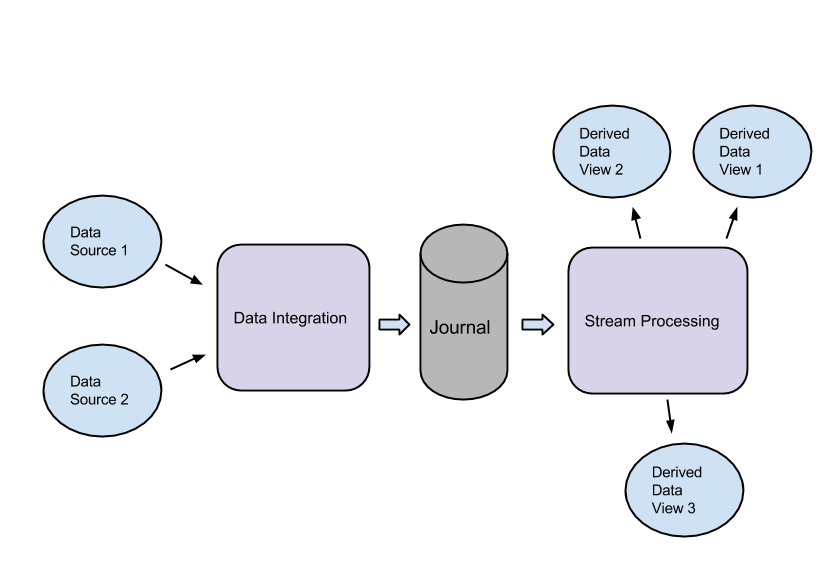
\includegraphics[width=1.0\textwidth]{img/main_archi.png}}
    \caption{Global architecture}
    \label{fig:main_archi}
  \end{center}
\end{figure}

Such an evented architecture allows easy decoupling of the write part (Data Integration) and the read part (Stream Processing),
but must be done with a lot of care concerning technical architecture.

The platform needs to do lot of IO in order to push the stream of events from data sources to data consumer, and must
parallelize a lot of operations. Moreover, it must ensure that the stream of events (producer) does not overwhelmed the stream
processors (consumers), i.e if consumers process data slowly, producer must try to slow the push rate. It should also deal with possible
failure of components and offer strong guarantees on these cases (like no message loss).

In order to fulfill those requirements, an asynchronous non-blocking approach will be taken to develop the platform in order to
minimize IO cost, decouple components, take easily advantage of parallelization and handle failure based on the 
Reactive Programming manifesto principles \cite{bib:reactiveManifesto}.










